\begin{refsection}
\chapter{Correcting optical imperfections in refractive lenses}\label{sec:corrections}

The necessity and possibility of arbitrarily manipulating the X-ray wavefront has been teased since, at least, the early 2000's [\cite{Chubar1999, Chubar2001b}]. It was not until the advent of extremely accurate additive and subtractive manufacturing techniques [\cite{Stohr2015, Polikarpov2016, Petrov2017, Roth2018, Sanli2018, Seiboth2019, Abrashitova2020, Antipov2020, Lin2020, Medvedskaya2020}] that the demonstration of free-form X-ray refractive optics was done [\cite{Sawhney2016,Seiboth2017,Laundy2019, Seiboth2020}]. The possibility of producing very accurate free-form optics for the correction of optical aberrations has brought renewed interest in wavefront sensing [\cite{Berujon2015, Seaberg2019}] and optical design simulations [\cite{Laundy2020}]. This chapter presents the early results on correcting optical imperfections in refractive lenses obtained at the ESRF. The design and expected performance is based on the lenses presented in \S\ref{sec:single_lens}~-~\textit{\nameref{sec:single_lens}} and the simulations shown in Chapter~\ref{sec:effect_optical_imperfections}~-~\textit{\nameref{sec:effect_optical_imperfections}}.

%-------------------------------------------------------------------------
%-------------------------------------------------------------------------
\section{Corrective optics}\label{sec:corrective_optics}
%-------------------------------------------------------------------------
%-------------------------------------------------------------------------

Correcting optical imperfections can be done by actively reshaping an optical element (adaptive optics) [\cite{Sutter2012, Alcock2013}] or by inserting a static (passive) optical element specially fitted to compensate the deviations from a perfect profile [\cite{Morawe2019}] or the wavefront error in relation to an idealised intensity [\cite{Donato2020}] or phase profile. Phase manipulation for wavefront manipulation can be done with diffractive elements [\cite{Probst2020}] or with refractive elements [\cite{Sawhney2016,Seiboth2017,Laundy2019,Seiboth2020}]. As indicated by the vast literature, refractive optics is the most popular method for correcting phase errors in partially-coherent X-ray beams. This section presents the design of refractive optical correctors for refractive lens stacks.

%-------------------------------------------------------------------------
%-------------------------------------------------------------------------
\subsection{Design}\label{sec:design}
%-------------------------------------------------------------------------
%-------------------------------------------------------------------------
\begin{figure}[t]
        \centering
        {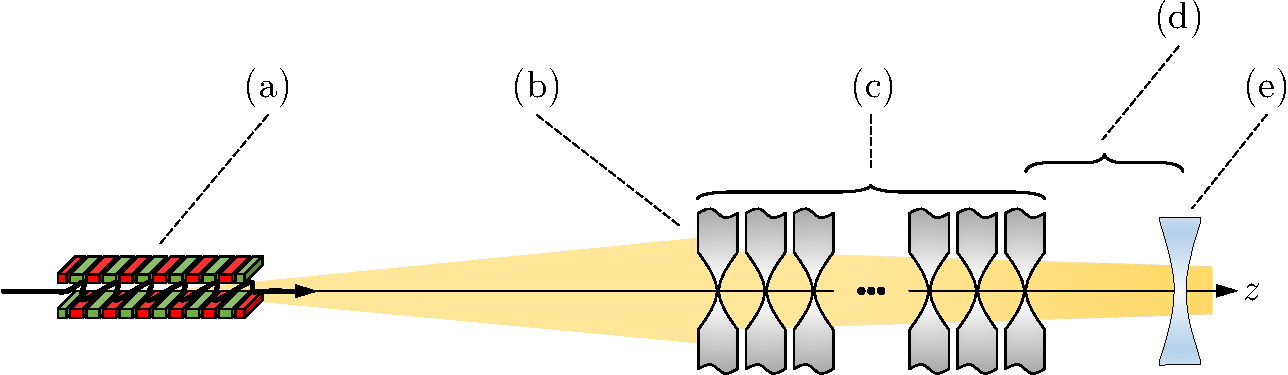
\includegraphics[width=0.6\linewidth]{figures/ch06/phase_extraction.pdf}}
        \caption[Schematic for phase correction calculation]{Schematic for residual phase extraction. (a) an arbitrary X-ray source delivers a (b) wave-field $U_{\text{illum.}}(x,y)$ immediately before the (c) optical system being studied. The wave-field exits the optical system and can be propagated a (d) distance $\Delta_{z_\text{pp}}$ from the exit pupil. At this position, the (e) extraction of the ideal phase from $U_{\text{exit}}(x,y)$ is done according to Eq.~\ref{eq:phase_corr}.}\label{fig:phase_extraction}
\end{figure}
Formally, the computation of the phase correction\footnote{The design of optical correctors for synchrotron radiation was first described in [\cite[\textit{§2}]{Chubar1999}], revisited in [\cite{Chubar2001b}] and first implemented for a 2D CRL in [\cite{Seiboth2017}].} for any optical system is done by assuming that the a wave-field will develop an specific phase $\phi_{\text{exit}}(x,y)$ distribution after passing through an arbitrary optical system. Ideally focusing a wave-field to a point-source at a distance $r$ from the exit pupil requires that that the developed phase $\arg [U_{\text{exit}}(x,y)]$ to be that of a spherical-wave as in Eq.~\ref{eq:spherical} [\cite{Chubar1999}]. Given the typical geometric apertures and focal distances of a CRL composed of few individual lenses\footnote{Assuming that the focusing inside the CRL is negligible - cf. [\cite{Schroer2005}] and [\cite[\textit{\S6}]{Seiboth2018}].}, it is possible use the phase of the paraxial approximation of Eq.~\ref{eq:spherical}, that is, the parabolic-phase of the wavefront in Eq.~\ref{eq:parabolic}. If the wavefront illuminating the optical system is given by $U_{\text{illum.}}(x,y)$, then, after passing through an aberrated lens system, $U_{\text{exit}}(x,y)$ is given by:
\begin{equation}\label{eq:U_exit}
    U_{\text{exit}}(x,y) =   \mathcal{D}(\Delta_{z_\text{pp}})\cdot\left[\mathrm{T}_{\text{CRL-MS}}(\Delta_z) \cdot U_{\text{illum.}}(x,y)\right],
\end{equation}
where $\mathcal{D}(\Delta_{z_\text{pp}})$ is a free-space propagation from the exit pupil of the optical system to the position along the optical axis where the phase correction is performed (Eq.~\ref{eq:Fresnel_operator}) and $\mathrm{T}_{\text{CRL-MS}}(\Delta_z)$ is the operator description of a lens stack given by Eq.~\ref{eq:TE_CRL_MS_ERR}. The phase shift necessary to correct such wavefront can be calculated as:
\begin{equation}\label{eq:phase_corr}
   \phi_{\text{correction}}(x,y) = \arg\left[\cfrac{\exp{\Big(-ik\frac{x^2 + y^2}{2z_f}\Big)}}{U_{\text{exit}}(x,y)}\right].
\end{equation}
Where $z_f$ is the distance from the phase corrector to the image plane [\cite{Seiboth2017}]. This phase extraction procedure is illustrated in Fig.~\ref{fig:phase_extraction}. A phase corrector based on refractive optics can be calculated directly from the phase obtained in Eq.~\ref{eq:phase_corr} and the transmission element in projection approximation phase-thickness relationship described by Eq.~\ref{eq:aux_funcs_transb}:
\begin{equation}\label{eq:phase_plate}
   \Delta_\text{pp}(x,y)=-\frac{\phi_{\text{correction}}(x,y)}{k\delta_\text{pp}(x,y)}.
\end{equation}
Where $\Delta_\text{pp}(x,y)$ is the local phase plate thickness in projection approximation and $\delta_\text{pp}$ is the refraction index decrement of the material used for correcting $ \phi_{\text{exit}}(x,y)$. The resulting correction plate described by Eq.~\ref{eq:phase_plate} is directly proportional to the phase errors at each $(x,y)$ coordinate pair. Typical error maps are shown in Figs.~\ref{fig:metrology_zernike_profiles}, \ref{fig:recovered_thickness}, \ref{fig:accumulated_profile_1}-\ref{fig:CDo}. Current micro- and nanofabrication techniques used for manufacturing X-ray optics\footnote{Current for micro- and nanofabrication of 3D structures include: } are capable of reproducing such intricate shapes with high spatial and depth resolution, however the use of such correction plate in an experimental setup is rather impractical due to the several degrees of freedom concerned when aligning it against the aberrated optical system. Furthermore, it has been observed that 2D lenses produced by (hot) embossing are dominated by spherical aberration terms (primary, secondary, tertiary...) and other azimuathally symmetric errors due to intrinsic manufacturing processes [\cite{Schropp2013, Uhlen2014, Seiboth2016, Seiboth2017, Celestre2020, Seiboth2020}] -  see also the Zernike polynomial bar plots (orange bars) in Figs.~\ref{fig:metrology_zernike_profiles}, \ref{fig:recovered_thickness}, \ref{fig:accumulated_profile_1}-\ref{fig:CDo}. Trading some of the correction accuracy for more practicality when employing the correction plate in a beamline, it is possible to obtain a correction profile by azimuthally averaging $\Delta_\text{pp}(x,y)$:
\begin{equation}\label{eq:phase_plate_r}
   \Delta_\text{pp}(r)=\cfrac{\displaystyle\int\limits_{0}^{2\pi}{\Delta_\text{pp}(r,\theta)r\text{d}\theta}}{\displaystyle\int\limits_{0}^{2\pi}{r\text{d}\theta}},
\end{equation}
where $r=\sqrt{x^2 + y^2}$ and $\theta=\arctan{\big(y/x\big)}$ are the transformation from Cartesian to polar coordinates. The correction plate as calculated by Eqs.~\ref{eq:phase_plate} and \ref{eq:phase_plate_r} is tailored for an specific set of lenses operating at a defined energy, as evidenced by $\delta_\text{pp}$. Although true that a correction plate design is suited to an specific lens combination, for a moderate number of lenses where the focusing inside the CRL can be neglected, it has been demonstrated that the correction plate can be used over a range of energies around the design energy $\text{E}_\text{design}$ as the index of refraction decrement $\delta$ is proportional to $\lambda^2$ [\cite[\textit{\S6}]{Seiboth2018}] - see also Fig.~\ref{fig:delta_correction_plate}. This can be done by shifting the plate along the optical axis closer or further away from the design position $\Delta_{z_\text{pp}}$ if the new operation energy is lower or higher than $\text{E}_\text{design}$. The same considerations on the beam chromaticity in \textit{Chromatic aberrations} in \S\ref{sec:CRL_performance}~-~\textit{\nameref{sec:CRL_performance}} apply to the phase correctors. 

%-------------------------------------------------------------------------
%-------------------------------------------------------------------------
\subsubsection*{Materials}
%-------------------------------------------------------------------------
%-------------------------------------------------------------------------

It is natural to envision adopting the same materials used in X-ray lenses for the phase correctors. As for the lenses, the material used for the phase plate is intimately connected to the manufacturing process. Phase plates for optical correction have been produced using fused silica [\cite{Seiboth2017}], diamond [\cite{Polikarpov2016, Antipov2020}] and sapphire [\cite{Lin2020}], manufactured with laser ablation or ion-beam lithography [\cite{Medvedskaya2020}] (subtractive manufacturing); and polymeric resists such as SU-8 (commonly used in LIGA [\cite{Nazmov2004}] and other polymeric lenses [\cite{Stohr2015}]) and the proprietary IP-S used in additive manufacturing via two-photon polimerisation [\cite{Petrov2017, Roth2018, Sanli2018, Abrashitova2020,Lin2020}]. 


% Due to the nature of the refractive index in the X-ray regime, this proposed correction inherently does not take into account the chromaticity in the X-ray beam - see also \textit{Chromatic aberrations} in \S\ref{sec:CRL_performance}~-~\textit{\nameref{sec:CRL_performance}}. Beacause CRLs in storage rings are often put after a monochromator - eg. Si(111) with $\Delta \text{E}/\text{E}\approx10^{-4}$), the effects of the beam bandwidth can be neglected. However, for SASE emission in XFELs without further conditioning of the beam, chromaticity can deteriorate the performance of the phase plates [\cite{Seiboth2014, Seiboth2018}].

%-------------------------------------------------------------------------
%-------------------------------------------------------------------------
\subsection{Correction phase plate calculation}\label{sec:cpp_calculation}
%-------------------------------------------------------------------------
%-------------------------------------------------------------------------

Applying the correction plate design methodology (Eqs.~\ref{eq:U_exit}-\ref{eq:phase_plate_r}) to the individually measured and artificially stacked lenses L01-L10, which have been studied in depth - see Table.~\ref{tab:CDn} and Figs.~\ref{fig:accumulated_profile_1}, \ref{fig:CDn_vs_CDnStack} and \ref{fig:CDnS}; it is possible to recover a phase plate that will improve the performance of that particular optical system. An optical corrector to be used 10~mm downstream the last lens of the stack, made of diamond and designed to operate at 8~keV is shown (cut) in Fig.~\ref{fig:plate_profile}. Due to the averaging in Eq.~\ref{eq:phase_plate_r}, the profile of the the corrective plate is smooth and does not have high spatial-frequency components. The obtained profile is similar to the ones reported in [\cite{Seiboth2017,Seiboth2018,Seiboth2020}], which were obtained for stacks composed of similar lenses. The correction plate was designed using diamond due to its relative large refractive index decrement $\delta_\text{C*}$ at the expense of a higher absorption, good thermal and mechanical properties and volume homogeneity which translates into low X-ray small angle scattering when compared to Beryllium lenses [\cite{Chubar2020}]. The aforementioned properties make diamond a very interesting material for (refractive) X-ray optics [\cite{Polikarpov2016b,ShvydKo2017}].

Using the optical setup shown in Fig.~\ref{fig:recovered_phase_corrected}, it is possible to recover the residual figure error profile shown in Fig.~\ref{fig:residual_profile}(a) and described in Table~\ref{tab:corrected}. The profiles in Fig.~\ref{fig:residual_profile}(b)-(c) are substantially changed from the Fig.~\ref{fig:accumulated_profile_1}(b)-(c). The polynomial fit in Fig.~\ref{fig:residual_profile}(b) has virtually no spherical aberration terms. The concentric rings from the pressing tool apparent in Fig.~\ref{fig:accumulated_profile_1}(c) are completely removed from the residual errors in Fig.~\ref{fig:residual_profile}(c). Figure~\ref{fig:recovered_phase_corrected}(d) reinforces the observation of the reduction in the figure errors by the use of a azimuthally symmetric phase plate. The radially symmetric components (orange bars) in Fig.~\ref{fig:recovered_phase_corrected}(d) are almost completely removed, while the purple bars remain almost unchanged. Finally, Fig.~\ref{fig:recovered_phase_corrected}(e) shows a residual profile that is several times smaller than the one in Fig.~\ref{fig:accumulated_profile_1}(e).

% could still be removed and increase further the quality of the correction plate. This residual profile, although several times smaller than the residual profile in Fig.~\ref{fig:accumulated_profile_1}(e)

\begin{figure}[t]
        \centering
        {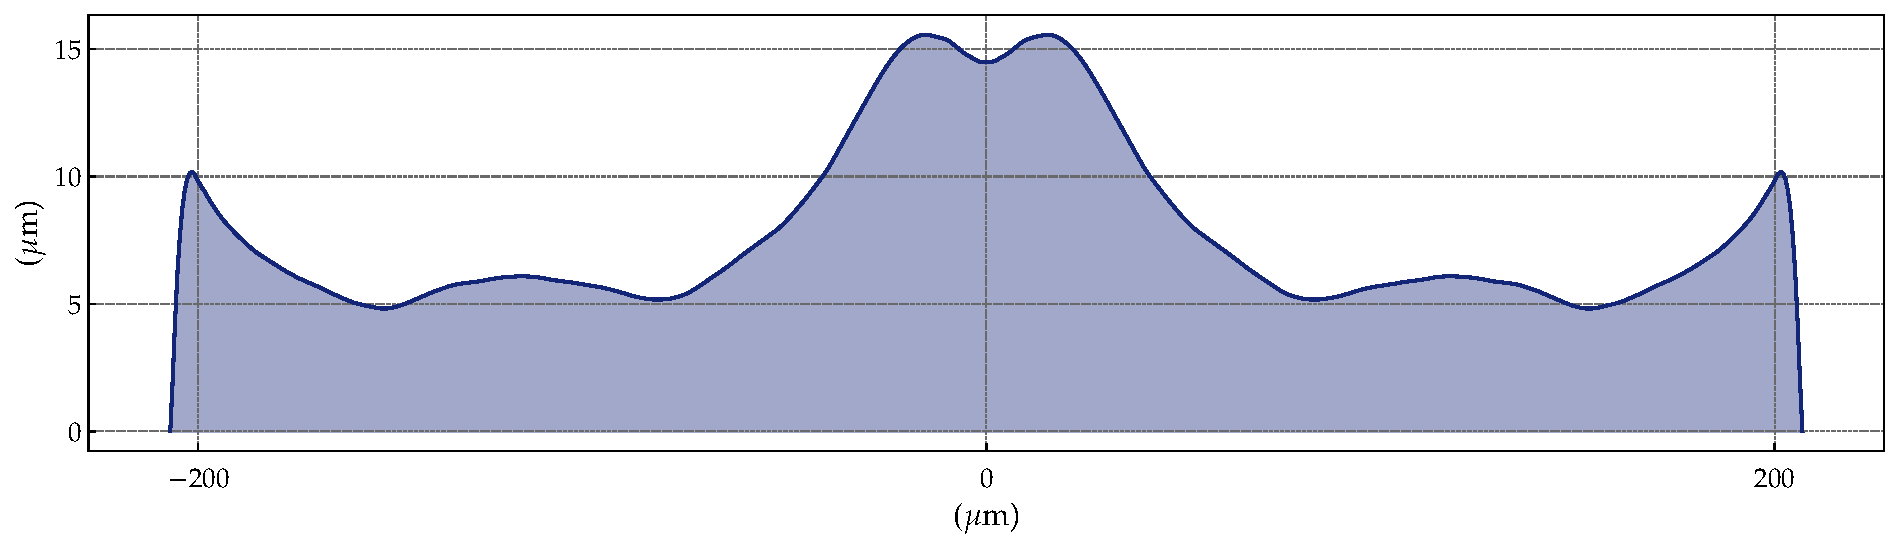
\includegraphics[width=0.6\linewidth]{figures/ch06/CDn_individual_8p0keV_n_10.0_lsp2p0mm_cpp10p0mm_phase_correction_plate_cut_2.pdf}}
        \caption[Diamond correction plate profile cut]{Profile cut of a diamond corrective plate for the lenses L01-L10 at 8~keV - cf. Fig.~\ref{fig:accumulated_profile_1}. The correction plate was calculated 10~mm downstream the exit pupil of the CRL.}\label{fig:plate_profile}
\end{figure}

\begin{figure}[t]
        \centering
        {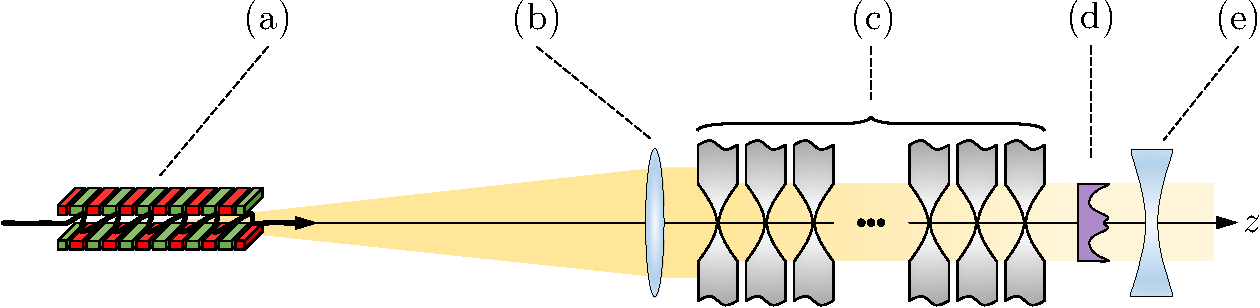
\includegraphics[width=0.6\linewidth]{figures/ch06/recovered_phase_corrected.pdf}}
        \caption[Schematic for residual thickness error calculation after phase correction]{Schematic for residual thickness error calculation after phase correction. (a) shows an arbitrary X-ray source. An (b) ideal parabolic phase element is placed downstream the radiation source to give the illumination a plane phase. The stacked X-ray lenses are placed immediately downstream. Any changes to the wave-field after (c) can be directly attributed to the the model under study. The phase plate is placed in (d) to correct the accumulated phase errors. An (e) ideal parabolic phase element with radius of curvature matching the developed quadratic term is then added and the residues (phase errors) can be extracted.}\label{fig:recovered_phase_corrected}
\end{figure}

\begin{figure}[t]
        \centering
        {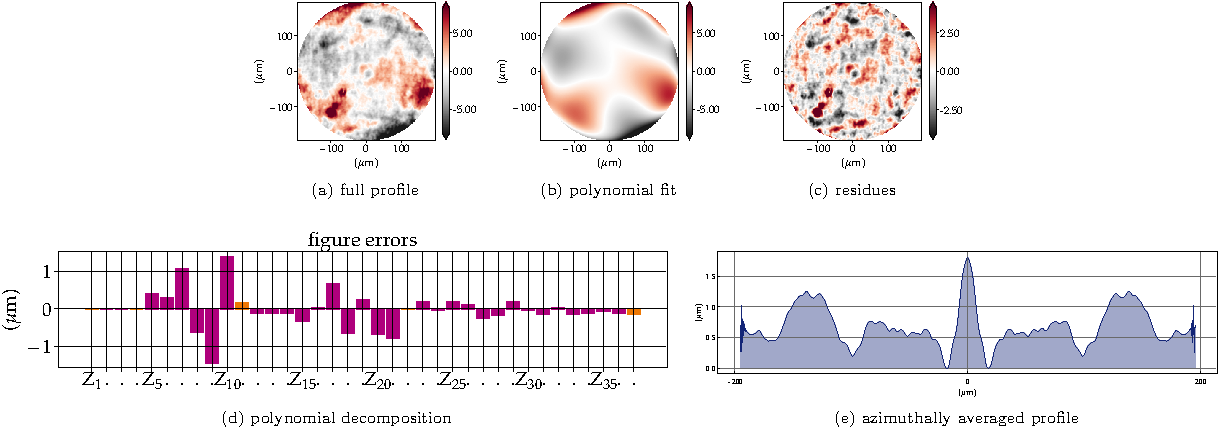
\includegraphics[width=1\linewidth]{figures/ch06/residual_profile.pdf}}
        \caption[Residual profile after phase correction]{Residual thickness error of the individually measured and artificially stacked lenses L01-L10 corrected with the diamond phase plate displayed in Fig.~\ref{fig:plate_profile}.}\label{fig:residual_profile}
\end{figure}

\begin{table}[h]
    \caption[Residual figure error profile r.m.s. value for L01-L10 and for the corrected system]{Residual figure error profile r.m.s. value for L01-L10 (Fig.~\ref{fig:accumulated_profile_1}) and for the corrected system (Fig.~\ref{fig:residual_profile}).}
    \centering
    \label{tab:corrected}\small
    \begin{tabular}{rccc}
    \hline \hline
    &\multicolumn{3}{c}{figure errors$^\dagger$ (r.m.s) $\mu$m}\\ \cline{2-4}
    &full profile & pol. fit   & residues \\ \hline
    L01-L10:      &4.84  &4.36  &2.18\\
    L01-L10 + PP: &3.27  &2.84  &1.63\\
    \hline \hline
    \multicolumn{4}{r}{\footnotesize{$^\dagger$ values given for $A_{\diameter}=400~\mu\text{m}$}}     
    \end{tabular}
\end{table}

\begin{table}[h]
    \caption[Strehl ratio for L01-L10 and for the corrected system]{Comparison of the Strehl ratio for aberrated system composed of L01-L10 and the corrected system as shown in Fig.~\ref{fig:Strehl_correction}.}\label{tab:Strehl_corrected}%\small
    \resizebox{\columnwidth}{!}{
    \centering
    \begin{tabular}{lrcccccc}\hline \hline
    &    &$\sigma_z$ ($\mu$m)     &$S_{\text{a}}$ (Eq.~\ref{eq:Strehl})  &$S_{\text{b}}$  (Eq.~\ref{eq:Marechal}) &$S_{\text{c}}$  (Eq.~\ref{eq:Mahajan}) &Coherent &Partially-coherent \\ \hline
    Fig.~\ref{fig:Strehl_correction} &L01-L10  &4.84  &0.067      &0.285 &0.393  &0.394          &0.409 \\
    &L01-L10 + PP                              &3.27  &0.503      &0.545 &0.608  &0.595         &0.671\\
    \hline \hline
    \end{tabular}
    }
\end{table}{}

%-------------------------------------------------------------------------
%-------------------------------------------------------------------------
\subsubsection*{Expected performance}
%-------------------------------------------------------------------------
%-------------------------------------------------------------------------

By reproducing the simulations from \S\ref{sec:coherent_sim}~-~\textit{\nameref{sec:coherent_sim}} and \S\ref{sec:partcoherent_sim}~-~\textit{\nameref{sec:partcoherent_sim}} to the corrected optical system as shown in Fig.~\ref{fig:optical_setups_corrected}, it is possible to evaluate the correction plate performance and study its effect in a coherent- and partially-coherent X-ray beam. Figure~\ref{fig:CDn_corrected} summarises the simulations and can be directly compared to Fig.~\ref{fig:CDnS} as it
shows the beam profile at selected positions up- and downstream the focal plane for a (a) partially- and for a (b) coherent beam. The beam caustics is shown in Fig.~\ref{fig:CDn_corrected}(c), while the (d) phase and (e) amplitude of the PSF, as well as the (f) source image are shown right next to it. A graphical representation of the Strehl ratio for the aberrated system and corrected system is shown in Fig.~\ref{fig:Strehl_correction} for the coherent and partially-coherent cases.

\begin{figure}[t]
        \centering
        {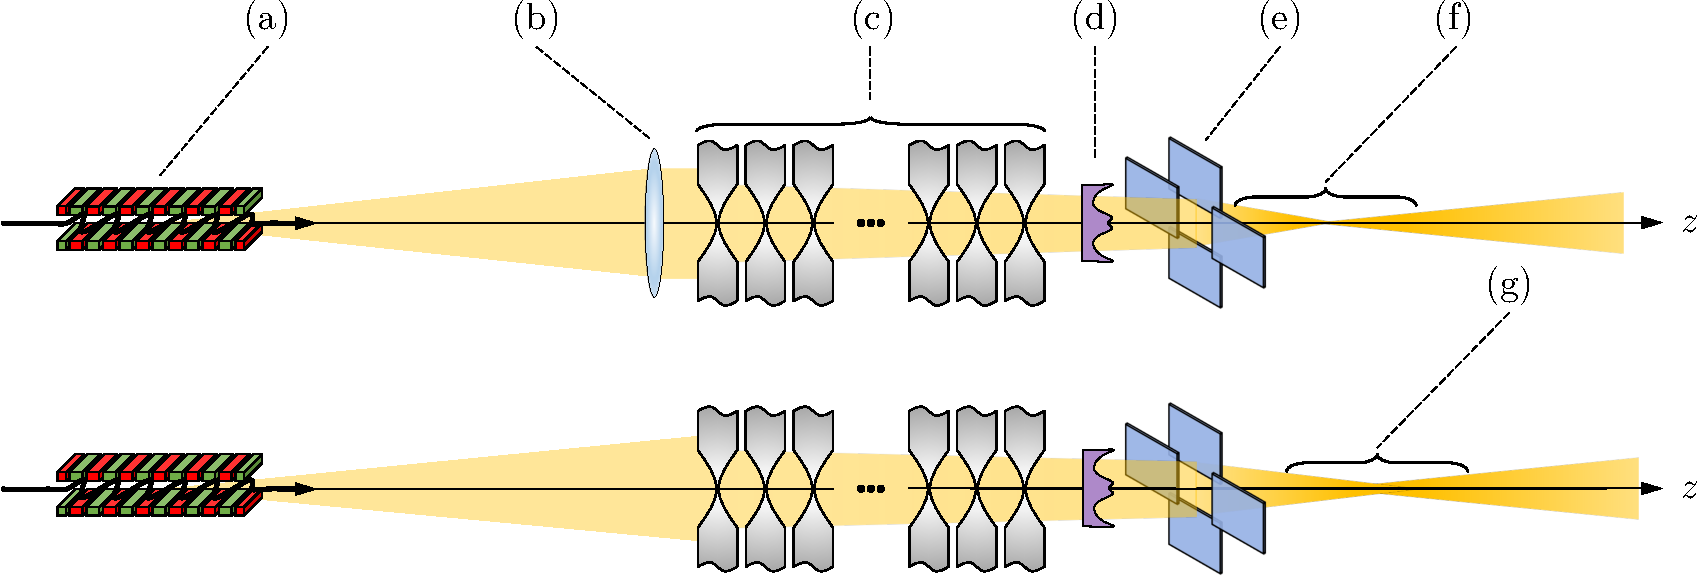
\includegraphics[width=0.8\linewidth]{figures/ch06/optical_setups_corrected.pdf}}
        \caption[Beamlines for coherent- and partially-coherent simulations]{\textbf{top row}: beamealine used for  \S\ref{sec:coherent_sim}~-~\textit{\nameref{sec:coherent_sim}}. \textbf{bottom row}: beamealine used for  \S\ref{sec:partcoherent_sim}~-~\textit{\nameref{sec:partcoherent_sim}}. (a) shows the X-ray source. An (b) ideal parabolic phase element is placed downstream the radiation source to give the illumination plane phase. This ideal element is only present for the fully-coherent simulations. The lenses being studied are shown in (c), which are followed by the (d) the correction plate. A set of (e) slits to ensure the same geometric aperture for all simulations. For the fully-coherent simulations, the beam-caustic range is shown in (f) and the PSF is calculated at the centre of it. For the partially-coherent simulations, the beam profile evolution along the optical axis is shown in (g) and the beam characteristics at the focal position are calculated at the its centre. 
        }\label{fig:optical_setups_corrected}
\end{figure}





\begin{figure}[h]
        \centering
        {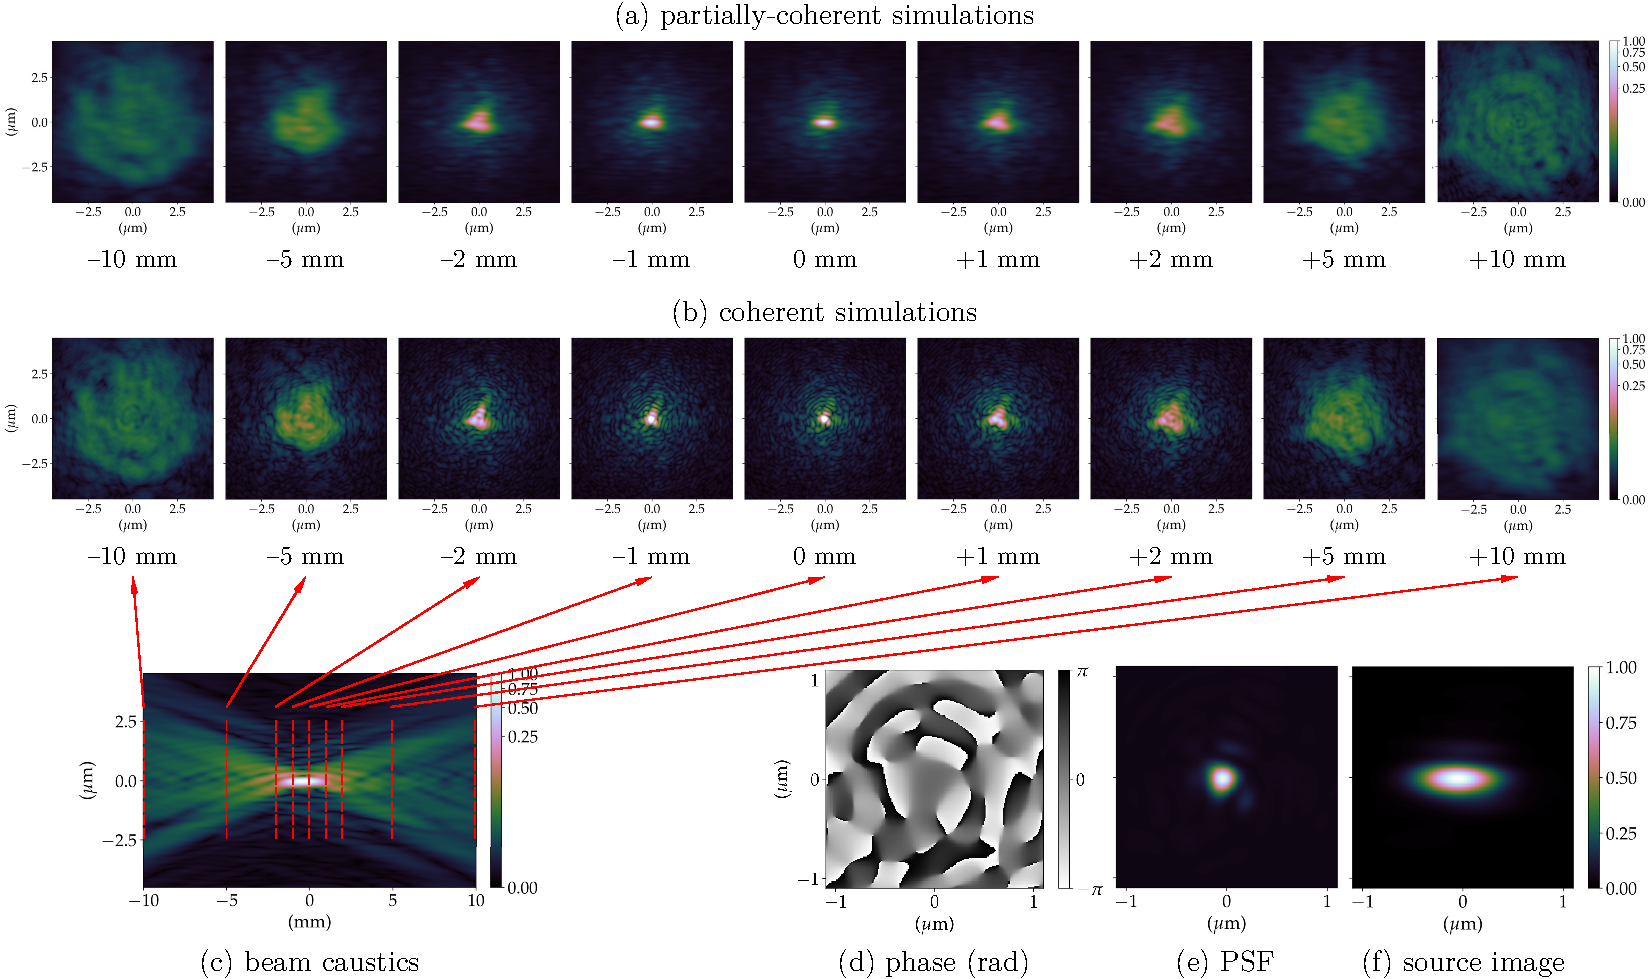
\includegraphics[width=0.99\linewidth]{figures/ch06/CDn_corrected.pdf}}
        \caption[Expected performance of the diamond phase corrector]{Expected performance of the Diamond phase corrector. (a) partially-coherent simulations show the beam profile up- and downstream the focal position averaging 10$^{4}$ wavefronts to simulate the radiation emitted by an undulator; (b) the coherent simulations show the beam profile of a plane wavefront being focused; (c) beam propagation near the focal position (beam caustics) for a fully coherent beam (horizontal cut around $y=0$); (d) phase and (e) intensity of the PSF calculated focusing a plane-wavefront; (f) demagnified image of the undulator photon-source (extended source). The phase-plate was designed in diamond and a cut is shown in Fig.~\ref{fig:recovered_phase_corrected}. The residual error profile after the correction is shown in Fig.~\ref{fig:plate_profile}.}\label{fig:CDn_corrected}
\end{figure}

\begin{figure}[h]
        \centering
        {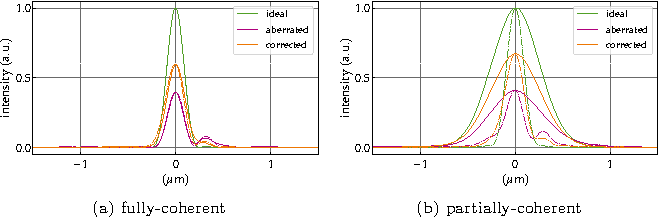
\includegraphics[width=0.7\linewidth]{figures/ch06/Strehl_correction.pdf}}
        \caption[Strehl ratio for the corrected system]{Visual representation of the Strehl ratio for the aberrated and corrected optical system. Coherent simulations are shown in (a) and partially-coherent simulations in (b) at 8~keV.}\label{fig:Strehl_correction}
\end{figure}

%-------------------------------------------------------------------------
%-------------------------------------------------------------------------
\subsubsection*{Tolerancing\footnote{This section came to be after some discussions with Andreas Schropp and Frank Seiboth (DESY, Germany) on the phase plate sensitivity to the alignment precision.}}
%-------------------------------------------------------------------------
%-------------------------------------------------------------------------

The expected performance of the correction plate shown in Figs.~\ref{fig:CDn_corrected} and \ref{fig:Strehl_correction} and compiled in the Tables~\ref{tab:corrected} and \ref{tab:Strehl_corrected} always assume that the phase plate is perfectly centred in respect to the optical axis, at the designed distance $\Delta_{z_\text{pp}}$ from the CRL and that it presents no tilt in relation to the optical axis. However, when mounting the phase-plate in a real experimental setup, these are very difficult to reproduce. To understand and establish the precision to which the alignment has to be done, a series of scans is presented in Fig.~\ref{fig:tolerancing}, which shows the simulations of a (a) longitudinal, a (b) transverse and an angular scan of the phase plate around its nominal (designed) position. The transverse alignment is clearly very important. The longitudinal alignment is, to a lesser extent, also important. The plate shows a relative insensitivity to angular misalignments. Although Fig.~\ref{fig:tolerancing} shows only coherent simulations, it is believed that the results can be applied to a moderately partially-coherent X-ray beam without great loss.

\begin{figure}[h]
        \centering
        {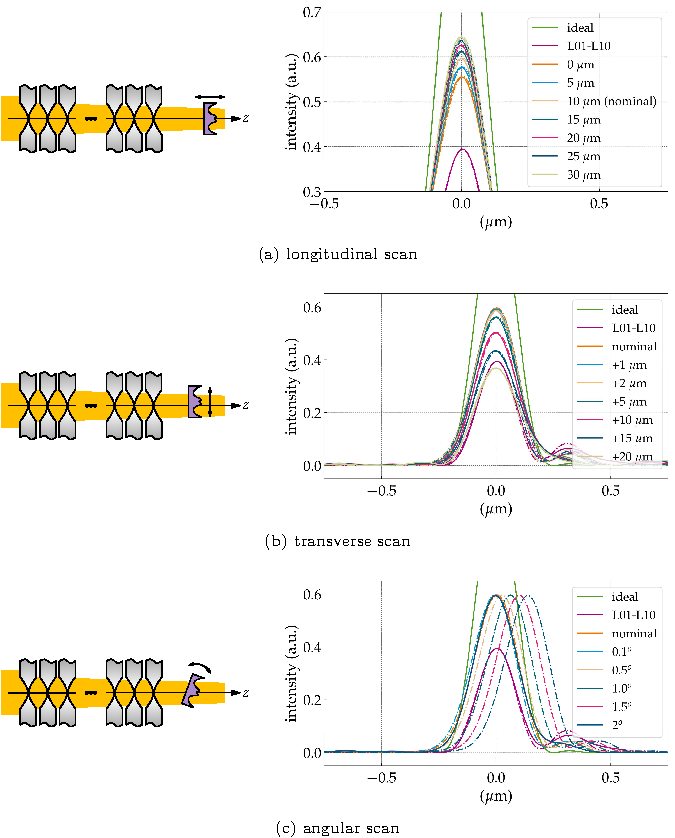
\includegraphics[width=0.6\linewidth]{figures/ch06/sensitivity_test.pdf}}
        \caption[Alignment sensitivity scan for the corrected system]{Study of the precision requeriments on (a) longitudinal, (b) transverse and (c) angular alignment of the phase plate.}\label{fig:tolerancing}
\end{figure}

\clearpage
%-------------------------------------------------------------------------
%-------------------------------------------------------------------------
\section{Prototype}\label{sec:prototype}
%-------------------------------------------------------------------------
%-------------------------------------------------------------------------

This section presents the early results 


%-------------------------------------------------------------------------
%-------------------------------------------------------------------------
\subsection{Early tests on an X-ray beam}\label{sec:prototype_testing}
%-------------------------------------------------------------------------
%-------------------------------------------------------------------------

%-------------------------------------------------------------------------
%-------------------------------------------------------------------------
\section{Discussion}\label{sec:corrective_optics_discussion}
%-------------------------------------------------------------------------
%-------------------------------------------------------------------------

The early results presented in are by no means discouraging. They there is a long way to reach results published by other groups, but they also indicate that the

$\blacksquare$

\clearpage
\addcontentsline{toc}{section}{References}
\printbibliography[heading=subbibliography]
\end{refsection}
